\documentclass{article}

\usepackage{graphicx}          % Para graficos
\usepackage{hyperref}          % Para meter hipervinculos
\usepackage{soul}
\usepackage{verbatim}

\graphicspath{ {./informe/images/} }

\begin{document}

\begin{titlepage}
  \vspace*{1cm}

  \begin{center}
    {\Huge{Trabajo Práctico 2: Software-Defined Networks}}
  \end{center}

  \vspace{0.4cm}

  \begin{center}
    {\LARGE{Facultad de Ingeniería de la Universidad de Buenos Aires}}\\
    \vspace{0.3cm}
    {\Large{Redes}}\\
    \vspace{0.3cm}
    {\large{Cátedra Hamelin-Lopez Pecora}}\\
  \end{center}

  \vspace{0.8cm}
  \begin{center}
    
\includegraphics[scale=0.8]{Logo-fiuba}
  \end{center}

  \vspace{1.4cm}
  \begin{center}

    {\begin{minipage}{.5\textwidth}
        \begin{center}
          Demarchi, Ignacio\\
          {\small{Padrón: 107835}}\\
          {\small{email: idemarchi@fi.uba.ar}}\\
        \end{center}
      \end{minipage}\begin{minipage}{.5\textwidth}
        \begin{center}
          Lijs, Theo\\
          {\small{Padrón: 109472}}\\
          {\small{email: tlijs@fi.uba.ar}}
        \end{center}
      \end{minipage}}

    \vspace{1.0cm}

    {\begin{minipage}{.5\textwidth}
        \begin{center}
          Schneider, Valentin\\
          {\small{Padrón: 107964}}\\
          {\small{email: vschneider@fi.uba.ar}}\\
        \end{center}
      \end{minipage}\begin{minipage}{.5\textwidth}
        \begin{center}
          Orsi, Tomas Fabrizio\\
          {\small{Padrón: 109735}}\\
          {\small{email: torsi@fi.uba.ar}}
        \end{center}
      \end{minipage}}

  \end{center}
\end{titlepage}

% \renewcommand*\contentsname{Indice}
\tableofcontents
\pagebreak

\section{Introducción}\label{introducciuxf3n}

En este trabajo practico se implemento la elaboracion de un SDN que, mediante OpenFlow (utilizando POX) implementa un Firewall sobre una red creada en Mininet.
Para poder ver el programa en accion y acercar la simulacion a un caso de uso real,
dentro de los hosts de la red de Mininet se utiliza iperf para establecer facilmente
una conexion entre clientes y servidores y ver el funcionamiento del Firewall en accion.
Para poder realmente ver esto, se utiiza Wireshark donde se observan los paquetes siendo enviados.


\section{Hipótesis y suposiciones realizadas - WIP}\label{hipuxf3tesis-y-suposiciones-realizadas-wip}

\newpage
\section{Herramientas utilizadas}\label{implementaciuxf3n-wip}
A continuacion se detalla el uso de cada herramienta ya mencionada para elaborar el trabajo practico.

\subsection{Mininet}\label{mininet}

Para utilizar Mininet, la topologia se define en mytopo.py. La misma recibe como
parametro la cantidad de switches a utilizar.

\begin{center}
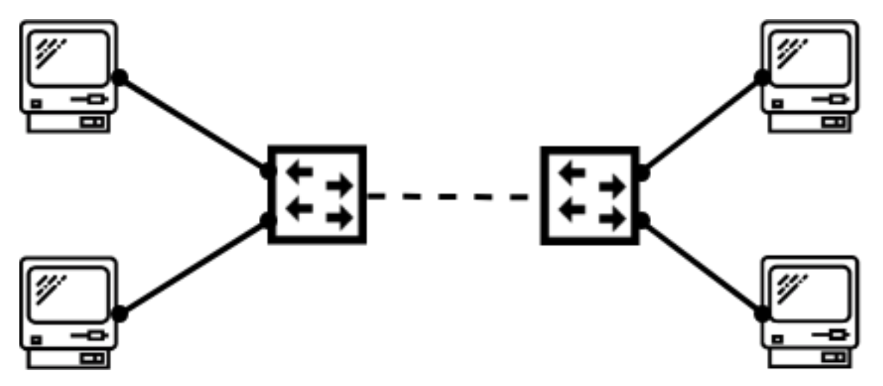
\includegraphics[scale=0.35]{images/mininet_topo.png}
\end{center}

Al correr el comando para levantar mininet, se establece la ip del controlador
que se va a utilizar. Esto es para que luego cuando corramos el controlador el mismo
pueda modificar los switches de la topologia y maneje el control plane de la red
de mininet.

\subsection{POX - WIP}\label{pox}
Para implementar el controlador con OpenFlow, se utilizo la biblioteca de POX.
El controlador utiliza l2 learning para que los switches aprendan automaticamente
a forwardear paquetes.
Para el firewall...
TODO: explicar como es que levanta y aplica las reglas, el formato de las reglas
y como conecta a lo que este corriendo en mininet

A continuacion se observa lo que el controlador loggea al iniciarse:
\begin{center}
 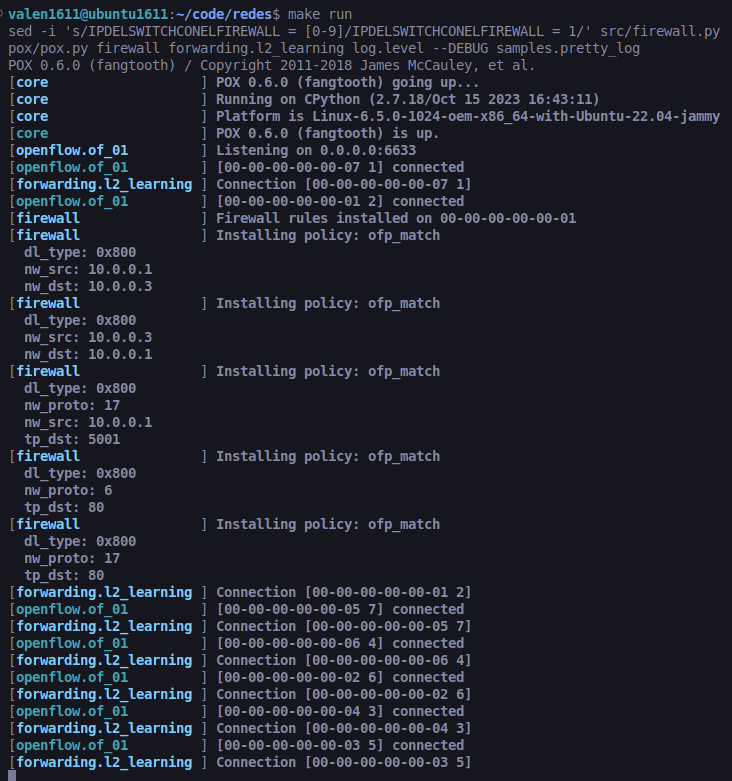
\includegraphics[scale=0.45]{images/pox_init.png}
\end{center}

\subsection{Wireshark \& iperf - WIP IMAGENES}\label{stop-and-wait}

Para comprobar el correcto funcionamiento de la red y del Firewall, se utiliza iperf para
simular clientes y servidores, y Wireshark para ver los paquetes enviados.

Al tener abierta la red de mininet, Wireshark la detecta como opcion para poder escuchar.

IMAGEN REDES QUE VE WIRESHARK
\begin{center}
% \includegraphics[scale=0.35]{wireshark_redes.png}
\end{center}

A continuacion se muestra el correcto funcionamiento del controlador, usando pingall dentro de mininet y escuchando con Wireshark.

\begin{center}
    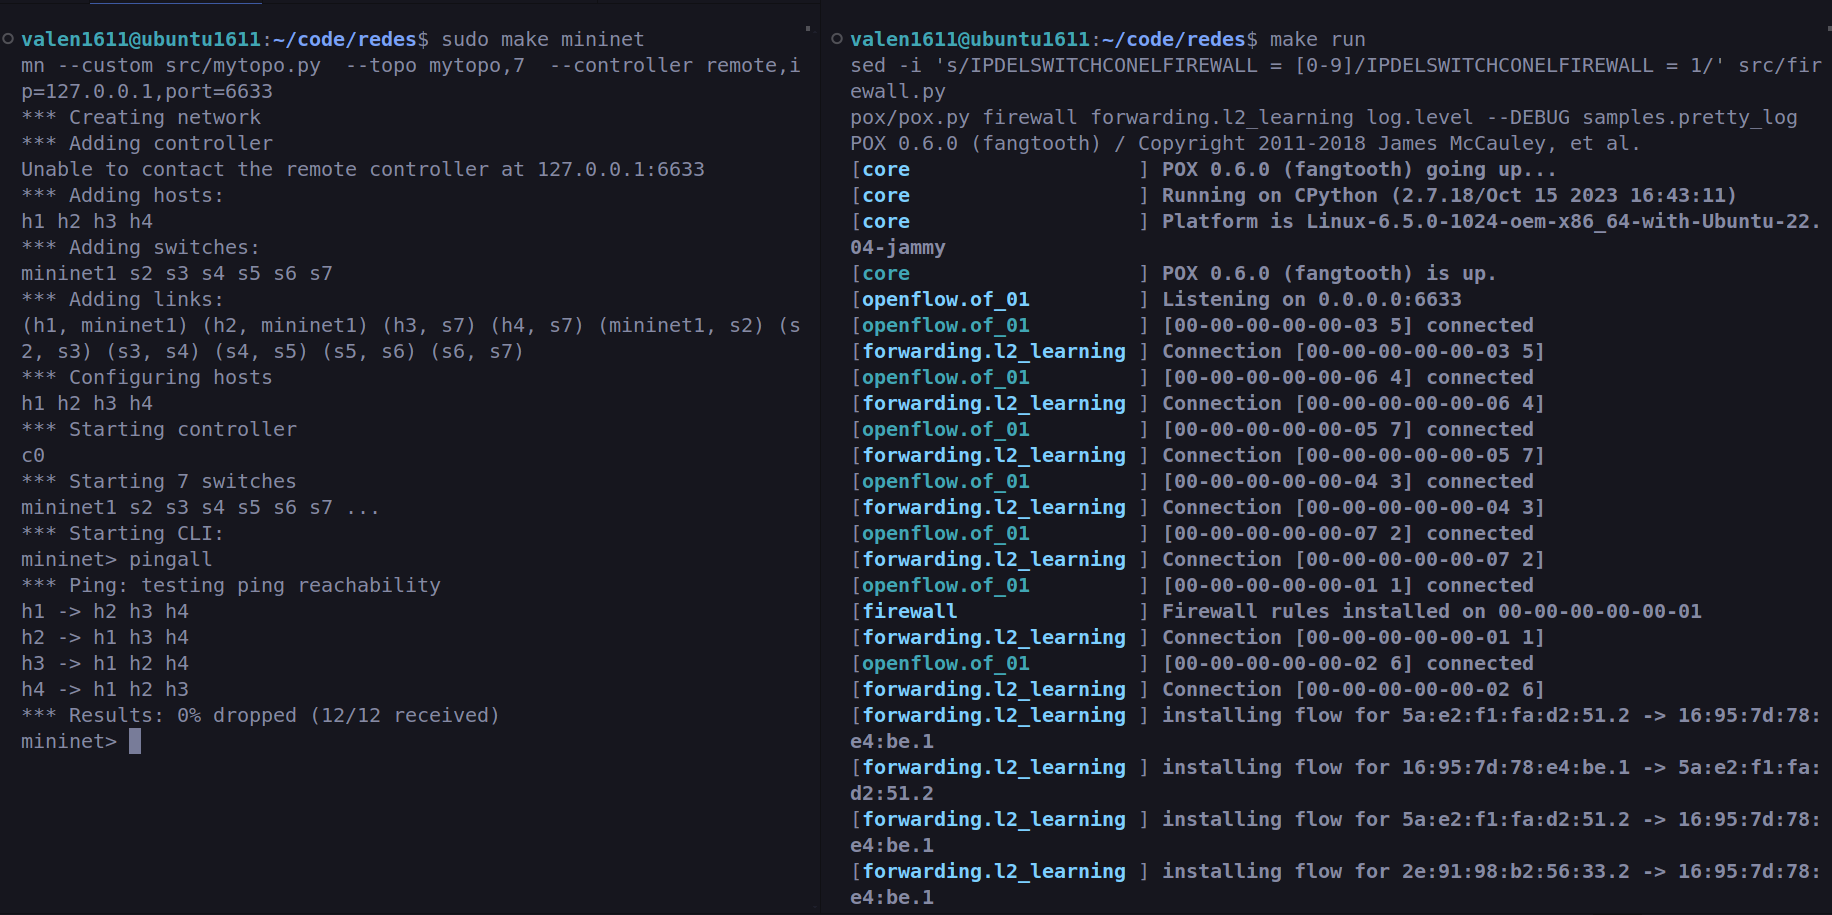
\includegraphics[scale=0.23]{images/mininet_pingall.png}
\end{center}

IMAGEN TRAZA WIRESHARK CON EL PINGALL DE MININET
\begin{center}
% \includegraphics[scale=0.5]{wireshark_pingall.png}
\end{center}


Para poder comprobar que no solo funciona con ICMP utilizamos iperf. Con iperf simulamos
clientes y servidores. En el ejemplo a continuacion tenemos al host h1 actuando como cliente
y al host h3 actuando como servidor, comunicandose por TCP.

\begin{center}
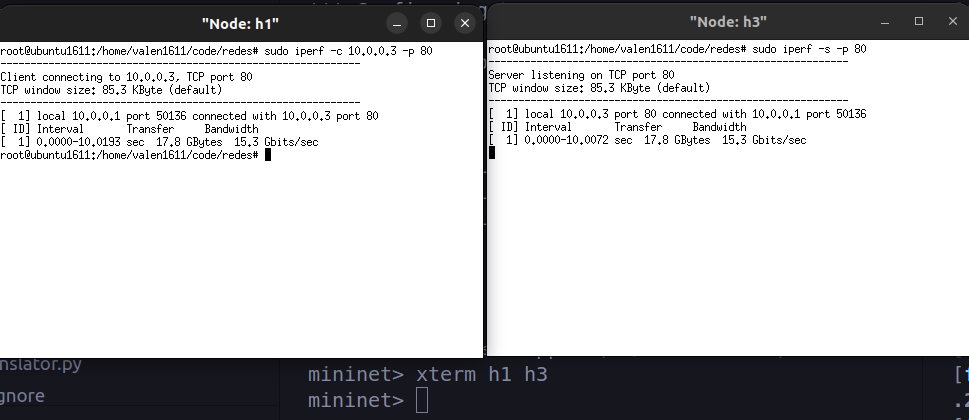
\includegraphics[scale=0.37]{images/mininet_iperf_basico.png}
\end{center}

IMAGEN TRAZA WIRESHARK CON EL IPERF BASICO
\begin{center}
% \includegraphics[scale=0.35]{wireshark_iperf_basico.png}
\end{center}

\newpage
\section{\texorpdfstring{\textbf{Resultados de simulaciones - WIP IMAGENES}}{Resultados de simulaciones}}\label{pruebas-wip}

\subsection{Puerto Destino 80}
Simulacion para descartar todos los mensajes cuyo puerto destino sea 80.

\subsubsection{Reglas}
\begin{center}
% \includegraphics[scale=0.35]{UploadJoseph.jpg(6,5MB)conStopWait}
\end{center}

\begin{verbatim}
{
    "policies":[
        {
            "dst_port": "80"
        }
]
}
\end{verbatim}


\subsubsection{Wireshark}
\begin{center}
% \includegraphics[scale=0.35]{UploadJoseph.jpg(6,5MB)conSelectiveRepeat}
\end{center}

\subsubsection{Logs del controlador}
\begin{center}
% \includegraphics[scale=0.35]{DownloadGrupo12.png(1,2MB)conStopWait}
\end{center}


\subsection{Host 1, Puerto 5001 y UDP}
Simulacion para descartar todos los mensajes que provengan del host 1, tengan como puerto destino el 5001, y esten utilizando el protocolo UDP.

\subsubsection{Reglas}

\begin{verbatim}
{
    "policies":[
    {
        "src_ip": "10.0.0.1",
        "dst_port": 5001,
        "protocol": "UDP"
    }
]
}
\end{verbatim}

\subsubsection{Wireshark}
\begin{center}
% \includegraphics[scale=0.35]{UploadJoseph.jpg(6,5MB)conSelectiveRepeat}
\end{center}

\subsubsection{Logs del controlador}
\begin{center}
% \includegraphics[scale=0.35]{DownloadGrupo12.png(1,2MB)conStopWait}
\end{center}

\subsection{Dos hosts no se comunican entre si}
Simulacion donde se eligen dos hosts cualquiera, y los mismos no pueden comunicarse de ninguna forma.

\subsubsection{Reglas}

\begin{verbatim}
{
    "policies":[
    {
        "banned_tuples": ["10.0.0.1","10.0.0.3"]
    }
]
}
\end{verbatim}


\subsubsection{Wireshark}
\begin{center}
% \includegraphics[scale=0.35]{UploadJoseph.jpg(6,5MB)conSelectiveRepeat}
\end{center}

\subsubsection{Logs del controlador}
\begin{center}
% \includegraphics[scale=0.35]{DownloadGrupo12.png(1,2MB)conStopWait}
\end{center}

\newpage
\section{\texorpdfstring{\textbf{Preguntas a responder}}{Preguntas a responder}}\label{preguntas-a-responder}

\subsection{1. ¿Cuál es la diferencia entre un Switch y un router? ¿Qué tienen en común?}\label{describa-la-arquitectura-cliente-servidor.}

La principal diferencia es que un switch opera en la capa 2 (enlace) y un router en la capa 3 (red).
Los switches redireccionan utilzando la direccion MAC de los dispositivos, mientras que los
routers utilizan la IP.

Lo que tienen en comun es que ambos funcionan para redireccionar paquetes y permitir
que hosts en distintas partes del mundo puedan comunicarse entre si.

\subsection{¿Cuál es la diferencia entre un Switch convencional y un Switch OpenFlow?}\label{detalle-el-protocolo-de-aplicaciuxf3n-desarrollado-en-este-trabajo.}

La diferencia mas importante entre un Switch convencional y uno OpenFlow es que el OpenFlow puede
ser gestionado mediante software con un controlador centralizado. Lo que permite automatizar
y agilizar el proceso.
Los switches convencionales no tienen el plano de control y el de datos desacoplados por lo que configurarlos requiere mas trabajo.

\subsection{¿Se pueden reemplazar todos los routers de la Intenet por Switches OpenFlow? Piense en el escenario interASes para elaborar su respuesta}\label{la-capa-de-transporte-del-stack-tcpip-ofrece-dos-protocolos-tcp-y-udp.-quuxe9-servicios-proveen-dichos-protocolos-cuuxe1les-son-sus-caracteruxedsticas-cuuxe1ndo-es-apropiado-utilizar-cada-uno}

En principio se podria, mas alla de incompatbilidades que podrian llegar a ser parcheadas. Pero no es algo factible realmente. Surgirian muchisimos problemas de seguridad, de rendimiento, de interoperabilidad, etc. En el contexto de interASes, si bien al manejar todo desde una misma tecnologia podria llegar a facilitar, por ejemplo, la implementacion de politicas de trafico para mejonar la flexibilidad de la gestion del mismo, se presentaria un single point of failure ya que todo dependeria de OpenFlow. Una vulnerabilidad que se descrubra sobre el protocolo en si dejaria expuesto a todo el internet global. Y dentro de una red privada, si no se tienen routers no podriamos utilizar NATs de la forma actual, habria que implementarla con los Switches. 

\section{Dificultades encontradas - WIP}\label{dificultades-encontradas}

\section{Conclusión - WIP}\label{conclusiuxf3n-wip}

\end{document}
